In the following subsections, each step of the planned refactoring presented in \autoref{sec:refactoring_plan} will be detailed, providing insights into the previous state of the project, and the results achieved though the refactoring.

\subsection{\texttt{logging} package refactoring}

Within this package, the \texttt{Logger} class supports four logging levels: \texttt{DEBUG}, \texttt{TRACE}, \texttt{AUDIT}, and \texttt{ASYNC\_ERROR}, which are defined in the \texttt{LoggingLevel} \texttt{Enum}. To enhance flexibility, the library maintains the current state of these logging levels in a \texttt{HashMap}, where each entry is represented as a record \texttt{<LoggingLevel, Boolean>}. In this mapping, the key corresponds to a specific logging level as an \texttt{Enum}, and the value is a boolean indicating whether that level is enabled.

The library also includes a test example that demonstrates how to extend the built-in logger by defining a \texttt{DescendantLogger} class, which extends the \texttt{Logging} class in order to support a new set of logging levels encoded as the \texttt{CustomLoggingLevel} \texttt{Enum}. However, since there is no inheritance between \texttt{CustomLoggingLevel} and \texttt{LoggingLevel}, the library requires creating a separate \texttt{HashMap} to store the new logging levels. This approach results in code duplication, as the \texttt{DescendantLogger} class must reimplement all methods for managing logging levels, such as enabling/disabling levels, checking if a level is enabled, and logging messages at specific levels. This violates the DRY (\href{https://en.wikipedia.org/wiki/Don%27\_repeat\_yourself}{Don't Repeat Yourself}) principle and increases the overall complexity of the codebase.

To address these design issues and create a more flexible and maintainable solution, a new abstract class, \texttt{BaseLogger}, was created. This class encapsulates the necessary data structures to manage any set of logging levels defined as \texttt{Enum} objects implementing the \texttt{ILoggingLevel} interface. This allows to store logging levels in a single \texttt{HashMap} regardless of their type, thus reducing code duplication and improving maintainability. Furthermore, a new generic interface, \texttt{ILogger<ILoggingLevel>}, was introduced. This interface includes a method, \texttt{log(String, ILoggingLevel)}, which is implemented by the \texttt{BaseLogger} class. This improved design is illustrated in \autoref{fig:refactored_logging}.

% Logging package original
\begin{minipage}{0.4\linewidth}
	\begin{figure}[H]
		\begin{center}
			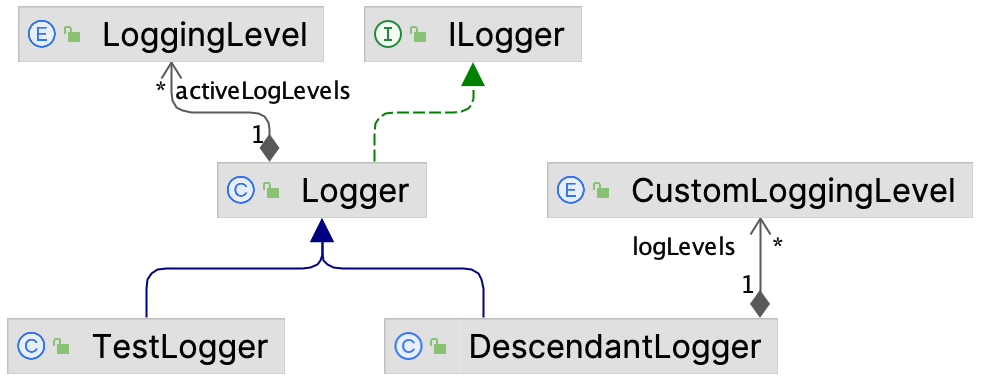
\includegraphics[width=0.95\textwidth]{figures/logging_package/original.png}
			\caption{Original \texttt{logging} package}
			\label{fig:original_logging}
		\end{center}
	\end{figure}
\end{minipage}
\begin{minipage}{0.6\linewidth}
	\begin{figure}[H]
		\begin{center}
			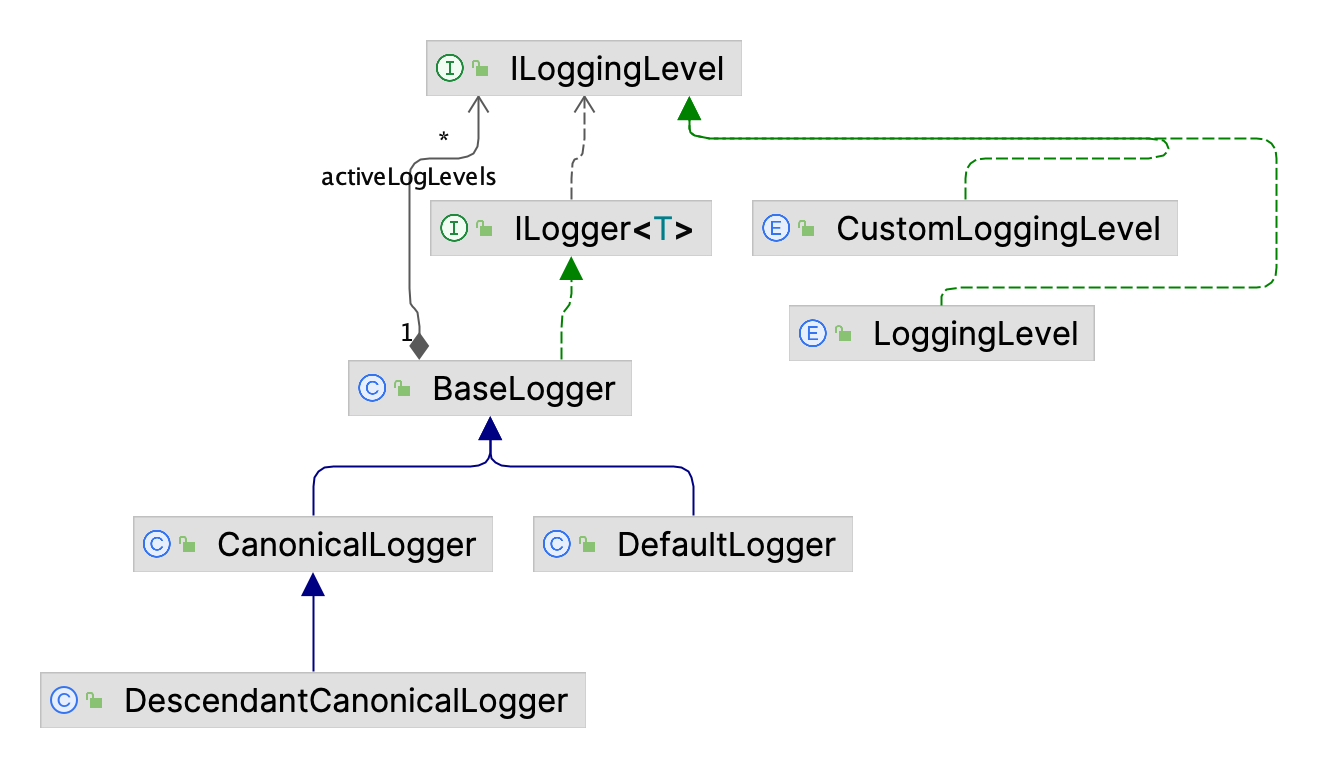
\includegraphics[width=0.95\textwidth]{figures/logging_package/refactored.png}
			\caption{Refactored \texttt{logging} package}
			\label{fig:refactored_logging}
		\end{center}
	\end{figure}
\end{minipage}

\noindent By adopting this approach, developers can define custom logger classes by simply creating new logging levels in an \texttt{Enum} that extends the \texttt{ILoggingLevel} interface. This eliminates the need to reimplement methods for managing logging levels or duplicating \texttt{HashMap} logic. As a result, the new architecture simplifies development and ensures adherence to the DRY principle.

As the \texttt{Logger} class was extensively used inside the core library, the refactoring process required updating all references to the \texttt{Logger} class to use the new \texttt{CanonicalLogger} class, which defines the default logging levels present in the original implementation to ensure backward compatibility. This was a long and tedious process, but it was necessary to ensure that the library maintained the same behavior as before.

Furthermore, also the proposed example of extension of the \texttt{Logger} class was refactored. Now, the \texttt{CanonicalLogger} class can be extended to support custom logging levels by simply defining a new \texttt{Enum} that implements the \texttt{ILoggingLevel} interface. This architecture allows an easy extension and customization of logging levels, as it is only necessary to define a new \texttt{Enum} that extends the \texttt{ILoggingLevel} interface and implement the required methods.

In the new test case, \texttt{DescendantCanonicalLogger} (previously \texttt{DescendantLogger}) implements an additional logging level \texttt{REQUEST} while still supporting the logging levels of the \texttt{CanonicalLogger} class. This demonstrates how the new architecture simplifies the process of extending the \texttt{Logger} class to support custom logging levels.

\subsection{Exception classes refactoring}

All exception classes are now in a single \texttt{exception} package in order to tidy up the codebase. The original design had exception classes scattered throughout the codebase, which made it difficult to locate and manage them.

\subsection{\texttt{queue} package refactoring}

The library defines a class \texttt{ActionQueue} that represents a queue of actions to be executed asynchronously by a thread. It receives a list of actions and executes them in the order they were added. For the development of the library, it was necessary to create a new class, \texttt{LoggingActionQueue}, which executes actions in a slight different way than \texttt{ActionQueue}. With the current architecture, \texttt{LoggingActionQueue} is almost an exact copy of \texttt{ActionQueue}. Refer to \autoref{fig:original_queue} for UML diagram of the original design.

To solve this issue, a new abstract class, \texttt{BaseActionQueue}, was created. This class encapsulates the common logic between \texttt{ActionQueue} and \texttt{LoggingActionQueue}, allowing to reduce code duplication and improve maintainability. After further analysis, was possible to remove completely the \texttt{LoggingActionQueue} class, as it was no longer necessary. The new design is illustrated in \autoref{fig:refactored_queue}.

% Logging package original
\begin{minipage}{0.5\linewidth}
	\begin{figure}[H]
		\begin{center}
			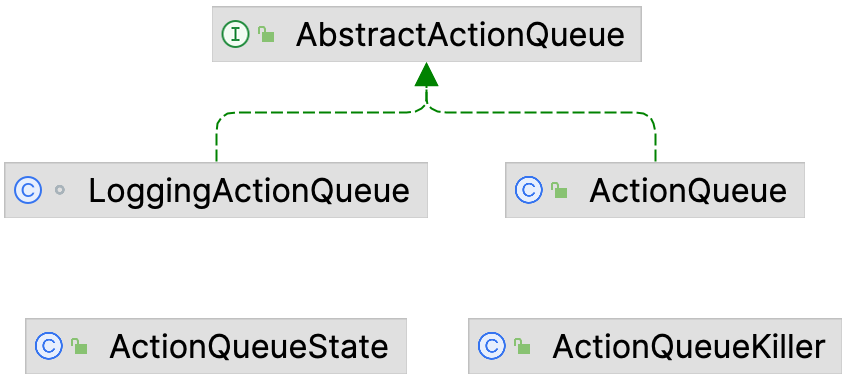
\includegraphics[width=0.95\textwidth]{figures/queue_package/original.png}
			\caption{Original \texttt{queue} package}
			\label{fig:original_queue}
		\end{center}
	\end{figure}
\end{minipage}
\begin{minipage}{0.5\linewidth}
	\begin{figure}[H]
		\begin{center}
			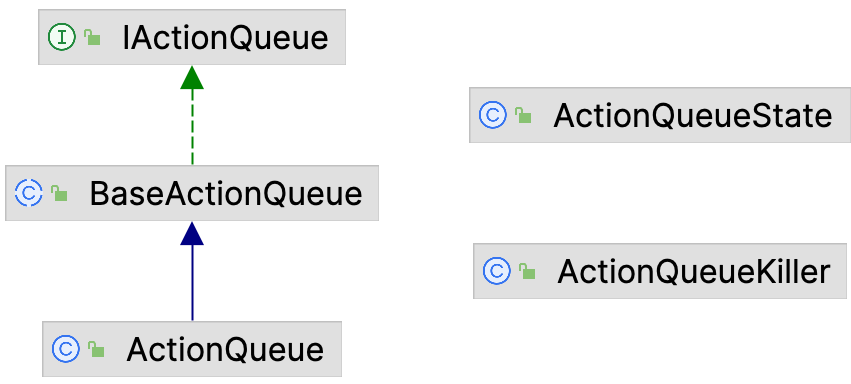
\includegraphics[width=0.95\textwidth]{figures/queue_package/refactored.png}
			\caption{Refactored \texttt{queue} package}
			\label{fig:refactored_queue}
		\end{center}
	\end{figure}
\end{minipage}

